\section{Important Concepts}

Before explaining the rules themselves, we will define several important concepts necessary for understanding the rulebook.

\subsection{Glossary}

\subsubsection{General}

\begin{description}
    \item[Codex:] A book describing the units, special rules, and history of a specific army, such as the Eldar Codex or Necron Codex.

    \item[Base:] A generic term representing either a group of 1--5 infantry miniatures or a single vehicle miniature. When the term \textit{base} is used in the rules, it refers to both the base and the miniatures mounted on it. Vehicle miniatures and larger models do not need to be mounted on bases.

    \item[Detachment:] A group of bases, generally consisting of 1--10 bases. Detachments have defined compositions listed in the Codexes. The detachment is the central element of the game. Orders are issued to detachments, activations are performed by detachment, morale applies to detachments, and bases belonging to the same detachment must remain in detachment coherency.

    \item[Formation:] To create an army list, each player purchases several formations. A formation consists of one or more detachments. The available formations are described in the Codexes.

    \item[Special Abilities:] Abilities possessed by certain units or weapons. Special abilities override the basic rules. The most common abilities are described in the rulebook, while abilities specific to a particular Codex are described in that Codex.

    \item[Objectives:] Objectives represent defensive positions, strategically important buildings, supply depots, and other important locations on the battlefield. They are represented by markers, and controlling them is important for winning the battle.

    \item[Template:] A game component, usually circular, used to represent the area of effect of certain weapons or abilities.
\end{description}

\subsubsection{Dice}

\begin{description}
    \item[Dice Roll:] Rolling one or more dice. Several types of dice rolls are used in the rules:
\end{description}

\begin{itemize}
    \item \textbf{D6:} Roll one six-sided die.
    \item \textbf{2D6:} Roll two six-sided dice and add their results together.
    \item \textbf{D3:} Roll one six-sided die, divide the result by two, and round up.
    \item \textbf{Scatter Die:} A die with four arrow faces and two ``Hit'' faces. A ``Hit'' result means that there is no scatter. Otherwise, the object scatters in the direction indicated by the arrow.
\end{itemize}

\begin{description}
    \item[Success Threshold:] Dice rolls often have a success threshold written as X+. Each die result equal to or greater than this threshold is a success.

    \item[Reroll:] Rolling one or more dice from a dice roll again. The rerolled results are final, even if they are worse than the original results. A rerolled die can never be rerolled a second time.
\end{description}

\subsection{Measurements}

In NetEpic, distances are measured from the centre of one base to the centre of another and are measured in centimetres. Pre-measuring is allowed without restriction.

\subsection{Detachment Coherency}

Bases belonging to the same detachment must remain close to one another. This is represented by \textit{detachment coherency}, which requires every base in the detachment to be no more than 6~cm from another base in that detachment. A detachment is in coherency if you can trace a path between any two of its bases through other bases in the detachment, with each base maintaining coherency.

Coherency must be maintained at all times, including while the detachment is moving. If a detachment is no longer in coherency, the separated parts of the detachment must attempt to rejoin during their next movement. The detachment is not required to restore coherency until it moves.

If this movement does not allow the separated parts to restore coherency, only one group is retained, chosen by the owning player. All other bases are immediately destroyed.

\begin{figure}
    \centering
    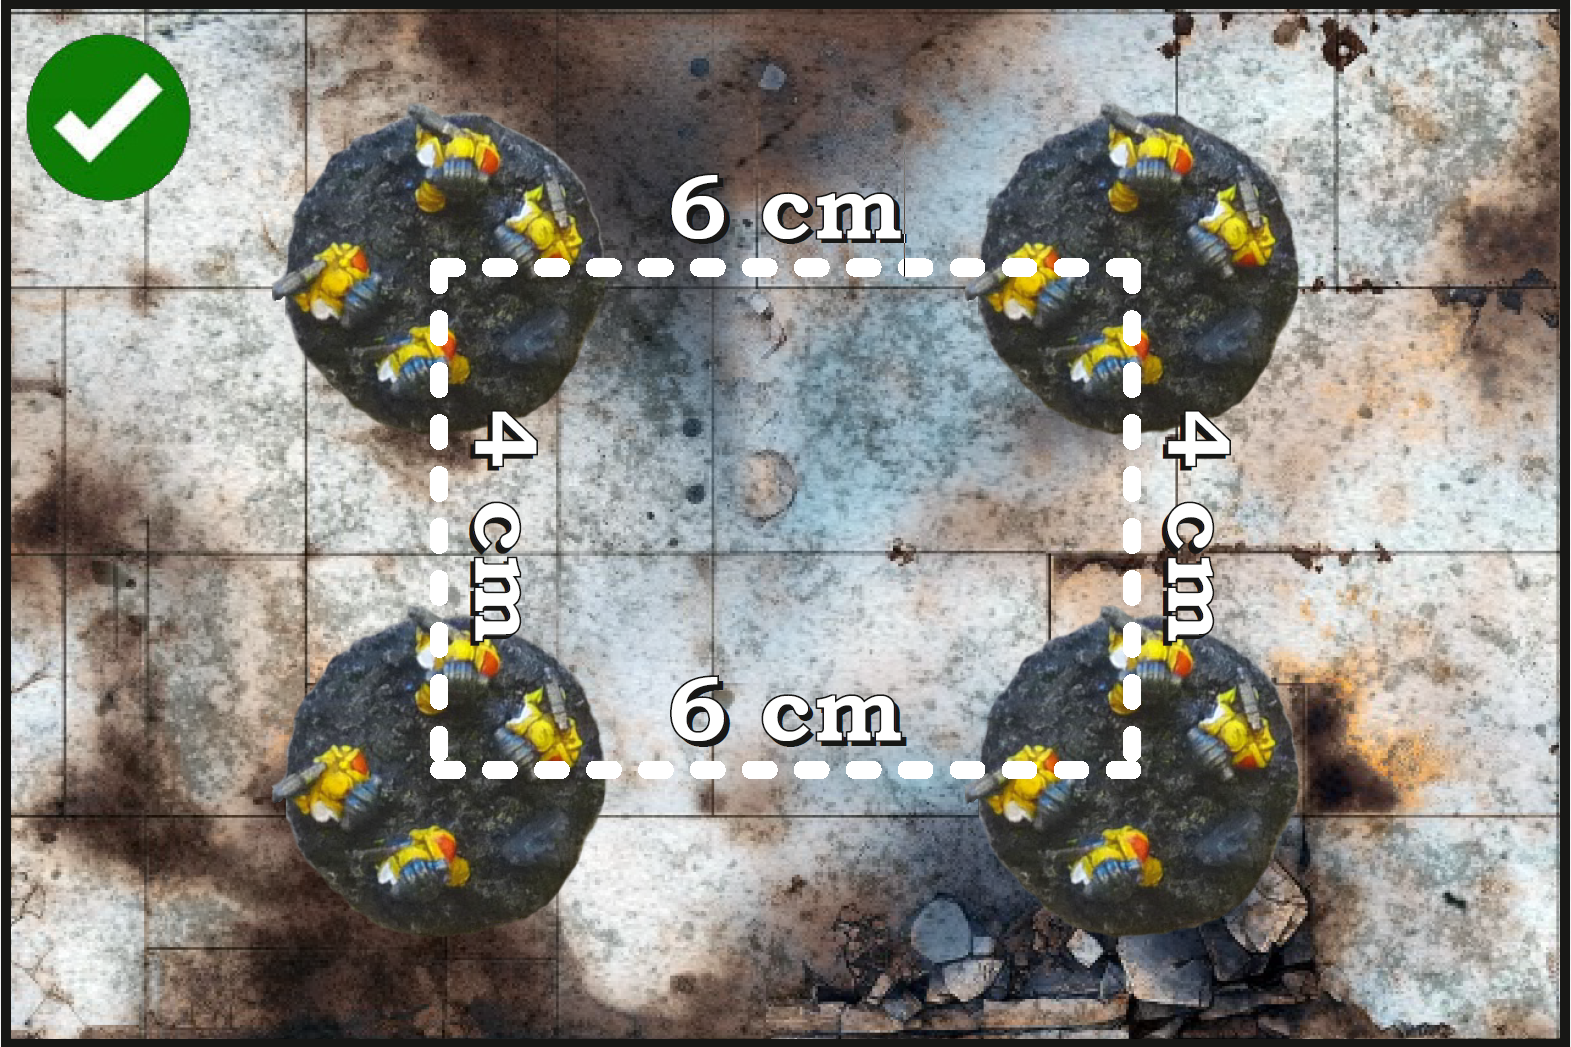
\includegraphics[width=0.5\linewidth]{00 - Intro/Coherency A.png}
    \caption{Detachment coherency is maintained in this example.}
    \label{fig:coherencyA}
\end{figure}
\begin{figure}
    \centering
    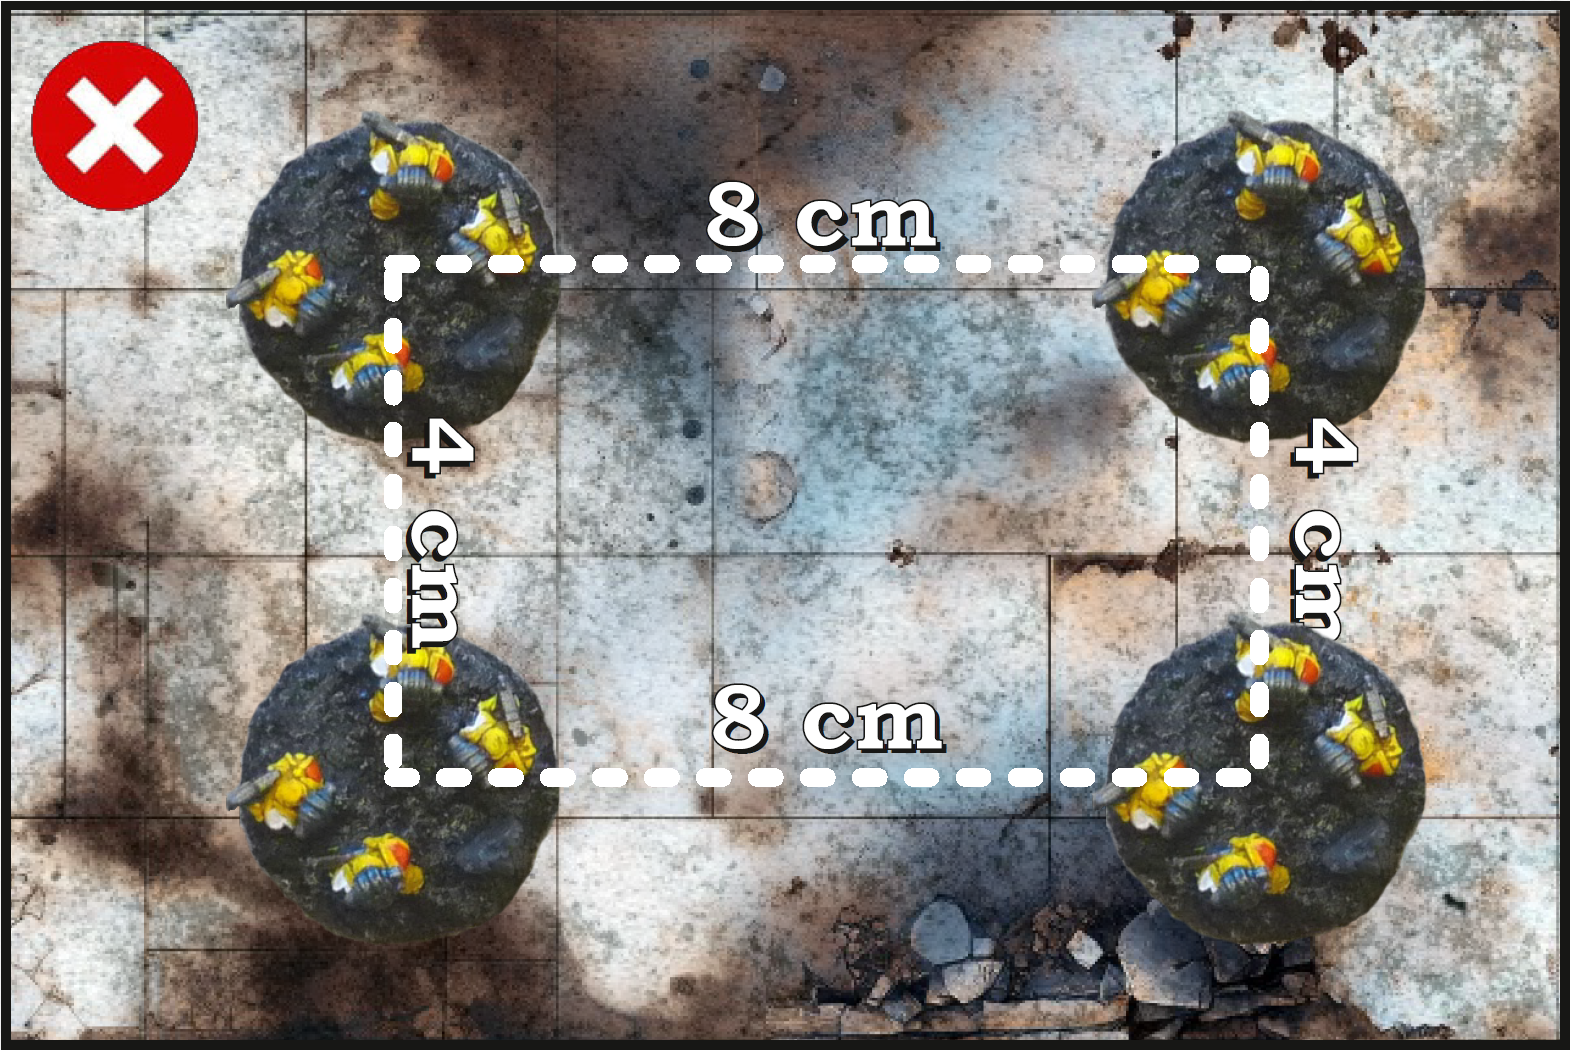
\includegraphics[width=0.5\linewidth]{00 - Intro/Coherency B.png}
    \caption{Detachment coherency is not maintained in this example, as the two groups are more than 6~cm apart.}
    \label{fig:coherencyB}
\end{figure}



\subsection{Class}

All bases have a class representing their size and mobility. The classes are:

\begin{itemize}
    \item \textbf{Class 1:} Infantry
    \item \textbf{Class 2:} Walkers and Cavalry
    \item \textbf{Class 3:} Vehicles
    \item \textbf{Class 4:} Super-heavy Vehicles and Knights
    \item \textbf{Class 5:} Titans / Light Praetorians
    \item \textbf{Class 6:} Titans / Battleline Praetorians
    \item \textbf{Class 7:} Titans / Heavy Praetorians
    \item \textbf{Class 12:} Altitude
\end{itemize}

\noindent\textbf{Pinned:} A base is pinned in an assault if it is engaged by an opponent of the same or a higher class. A pinned base loses its order and cannot move or fire. However, it may be activated during the Movement Phase if it has abilities or psychic powers that can be used.

\subsection{Zone of Control}

A base represents a threat to the area around it, represented in the game by its \textit{zone of control}. It is centred on the centre of the base and has a diameter of:

\begin{itemize}
    \item 7.5~cm for Class 1--4 bases.
    \item 12~cm for Class 5 and higher bases.
\end{itemize}

For game purposes, a base must be no larger than its zone of control.

A base loses its zone of control in the following circumstances:

\begin{itemize}
    \item If it is pinned in an assault.
    \item If it has engaged an enemy base in an assault.
    \item If it is immobilised.
    \item If it has a Fall Back order.
\end{itemize}

\subsection{Interdiction Zone}

The interdiction zone represents a base's long-range threat and affects certain aspects of the game for opposing bases, such as morale. It extends 25~cm around the base. A base does not generate an interdiction zone if it has a Fall Back order or is at altitude.

\subsection{Immobilised Base}

Immobilised bases can no longer move, change their facing, or consolidate an assault. They also lose their zone of control and roll 1D6 fewer in assaults.

\subsection{Altitude}

Bases at altitude are treated as Class 12 for line-of-sight purposes. During their movement, they ignore enemy zones of control and terrain features.

\subsection{Scatter}

An action that scatters, such as movement or shooting, requires a roll of the scatter die to determine its direction. If a ``Hit'' is rolled, the action does not scatter. Otherwise, it scatters in the direction indicated by the arrow. The distance is specified by the rule that caused the scatter.

\subsection{Front and Rear Arcs}

A base has a front arc covering the 180\textdegree{} area in front of it and a rear arc covering the 180\textdegree{} area behind it.

\subsection{Unit Profile}

A unit profile represents the characteristics of the relevant unit. It contains the following information:

\begin{description}
    \item[Name:] The name of the unit.

    \item[Movement:] The distance the base can normally move.

    \item[Save:] The unit's resistance to damage.

    \item[AF (Assault Factor):] The unit's strength in an assault.

    \item[Morale:] The base's ability to resist fear and avoid fleeing.

    \item[Weapons:] The name of the unit's weapon. If the unit has multiple weapons, each weapon has its own entry.

    \item[Range:] The distance at which the weapon can fire.

    \item[Dice:] The number of attack dice rolled by the weapon.

    \item[To Hit:] The result required on each attack die for the attack to succeed. Each success inflicts one hit on the target.

    \item[AP (Armour Penetration):] The weapon's ability to penetrate armour.

    \item[Abilities:] A list of the unit's special abilities.
\end{description}

\begin{table}[ht]
    \centering

    \begin{tblr}{
        colspec={
            Q[c,m,2] Q[c,m,1.5] Q[c,m,0.7] Q[c,m,0.9]
            Q[c,m,3.5] Q[c,m,1.3] Q[c,m,1.5] Q[c,m,2] Q[c,m,0.9]
        },
        cells={
            halign=c,
            valign=m
        },
        hlines,
        vlines,
        row{1}={
            bg=black,
            fg=white,
            font=\bfseries,
            ht=9mm
        }
    }
        Movement &
        Save &
        AF &
        Morale &
        Weapons &
        Range &
        Dice &
        To Hit &
        AP
        \\

        10~cm &
        5+ &
        $+2$ &
        5 &
        Bolters &
        45~cm &
        1 &
        5+ &
        0
    \end{tblr}
\end{table}

